\section{Auswertung}
\label{sec:Auswertung}
Die gemessenen Werte sind in den folgenden Tabellen dargestellt.

\begin{table}[H]
  \centering
    \caption{Die Messwerte der Amplitude der gedämpften Schwingung bei 826Hz.}
    \label{tab:messung1}
    \sisetup{table-format=3.1}
    \begin{tabular}{S S}
      \toprule
      {t/\si{\second}} & {Amplitude/\si{\volt}} \\
      \midrule
      0	   &  16.5 \\
      100	 &  12   \\
      200	 &  8  \\
      300	 &  5  \\
      400	 &  4  \\
      500	 &  3  \\
      600	 &  2  \\
      \bottomrule
    \end{tabular}
\end{table}

\begin{table}[H]
  \centering
    \caption{Die Messwerte der Amplitude der gedämpften Schwingung bei 1057Hz.}
    \label{tab:messung2}
    \sisetup{table-format=3.1}
    \begin{tabular}{S S}
      \toprule
      {$t/\si{\second}$} & {Amplitude/$\si{\volt}$} \\
      \midrule
        0	 &    18.0 \\
       20  &  	17.0 \\
       40  &  	15.5 \\
       60  &  	14.5 \\
       80  &  	13.0 \\
       95  &  	12.5 \\
      115  &    11.5 \\
      135  &  	10.5 \\
      155  &  	10.0 \\
      173  &  	 9.0 \\
      190  &  	 8.5 \\
      210  &  	 8.0 \\
      230  &  	 7.5 \\
      250  &  	 7.0 \\
      270  &  	 6.2 \\
      290  &  	 6.0 \\
      310  &     5.5 \\
      327  &  	 5.0 \\
      345  &  	 4.8 \\
      365  &  	 4.5 \\
      385  &  	 4.0 \\
      405  &  	 4.0 \\
      422  &     3.6 \\
      440  &  	 3.3 \\
      460  &     3.0 \\
      \bottomrule
    \end{tabular}
\end{table}

\begin{table}[H]
  \centering
    \caption{Die Messwerte der Erreger- und Kondensatorspannung bei verschiedenen Frequenzen des Serienresonanzkreises.}
    \label{tab:messung3}
    \sisetup{table-format=3.1}
    \begin{tabular}{S S S}
      \toprule
      { $\nu/\si{\kilo\hertz}$} & {$U/\si{\volt}$} & {$U_C/\si{\volt}$}  \\
      \midrule
      100	 &  8.5  &	-0.5   \\
      150	 &  9.0  &	-0.17  \\
      200	 &  9.0  &	-0.050 \\
      250	 &  9.0  &	-0.010 \\
      300	 &  9.0  &	 0.036 \\
      350	 &  9.0  &	 0.050 \\
      400	 &  9.0  &	 0.060 \\
      450	 &  9.0  &	 0.070 \\
      500	 &  9.0  &	 0.075 \\
      \bottomrule
    \end{tabular}
\end{table}

\subsection{Der gedämpfte Schwingkreis}
Zu den Messungen der Amplituden sind in folgenden Abbildungen die Einhüllenden dargestellt.

\begin{figure}[H]
  \centering
  \begin{subfigure}{\textwidth}
    \centering
    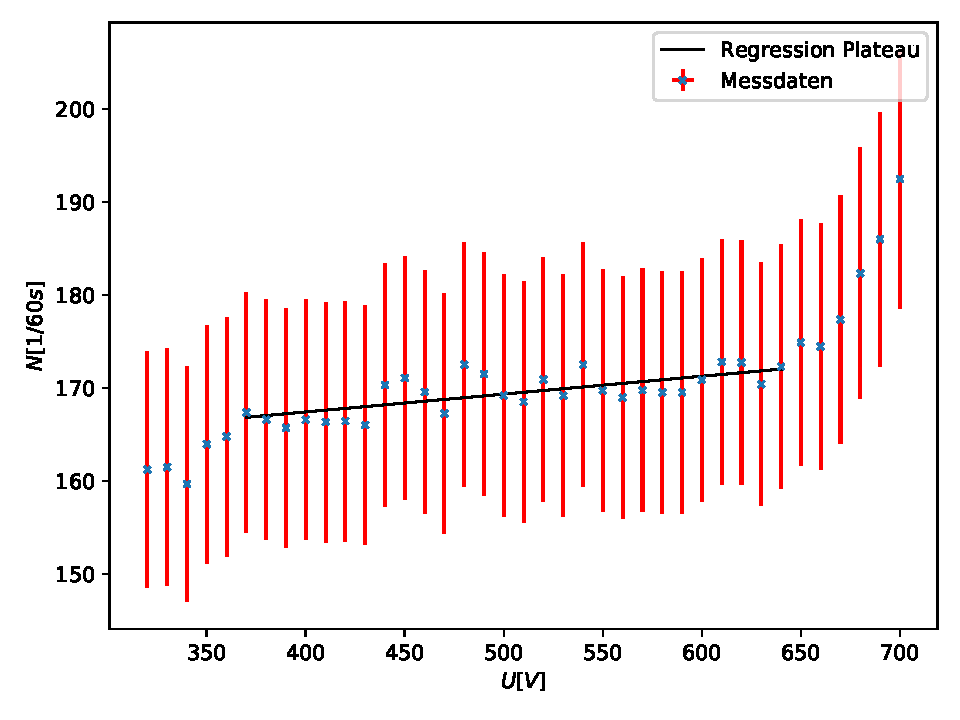
\includegraphics[scale=0.7]{auswertung/plot1.pdf}
    \caption{Die Einhüllende der zu \ref{tab:messung1} gehörenden Schwingungskurve.}
    \label{fig:plotmessung1}
  \end{subfigure}
  \begin{subfigure}{\textwidth}
    \centering
    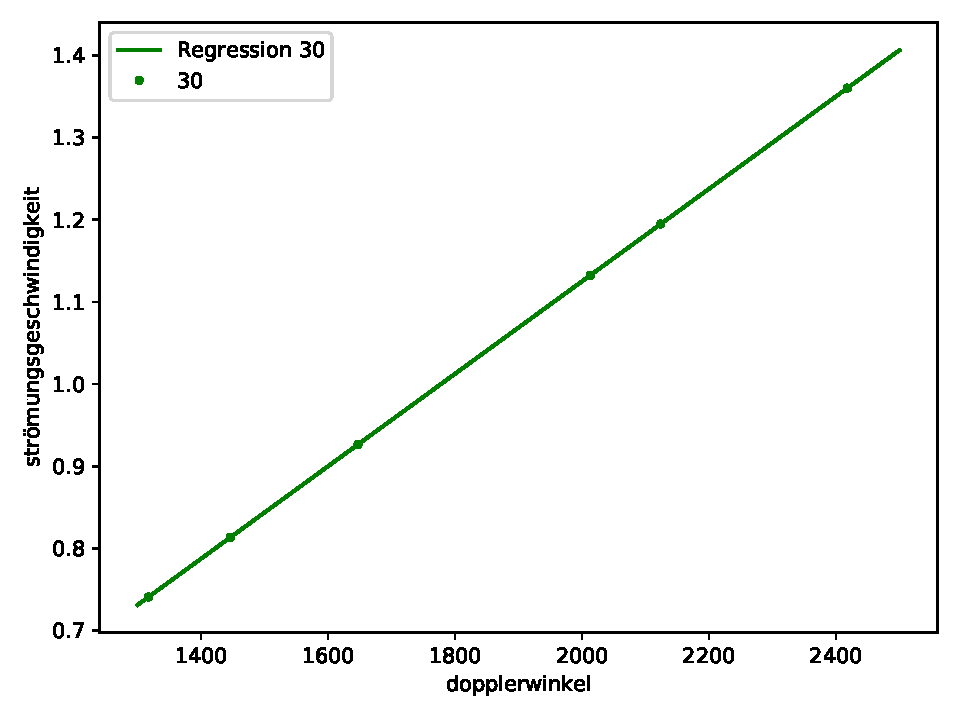
\includegraphics[scale=0.7]{auswertung/plot2.pdf}
    \caption{Die Einhüllende der zu \ref{tab:messung2} gehörenden Schwingungskurve.}
    \label{fig:plotmessung2}
  \end{subfigure}
\end{figure}
\noindent

Für die Messung \ref{tab:messung2} wurde eine Ausgleichsrechnung auf Basis einer e-Funktion mit negativem Exponeten durchgeführt. Dies wurde mit \textit{numpy} berechnet.
In folgender Abbildung sind die Regression sowie die ihr zu Grunde liegenden Daten visualisiert.

\begin{figure}[H]
  \centering
  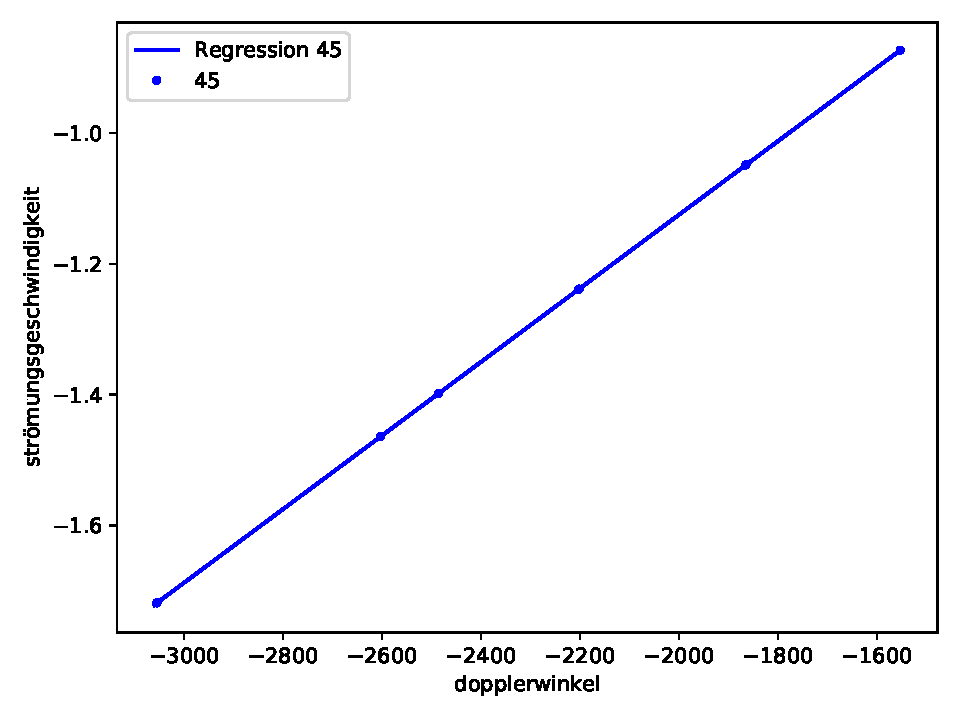
\includegraphics[scale=0.7]{auswertung/plot3.pdf}
  \caption{Die Regression auf Basis der Messung \ref{tab_messung2}.}
  \label{fig:regrmessung2}
\end{figure}

Die Regression wurde auf Basis folgender Funktion durchgeführt:

\begin{equation*}
  r(t) = A \cdot e^{-B t}
\end{equation*}

mit den Parametern

\begin{align*}
  A  = & 18.070 \pm  0.079 \\
  B  = & 0.004 \pm 2.912 \cdot 10^{-5}. \\
\end{align*}

Aus diesem Parameter $B$ lässt sich mit \eqref{eqn:Losung1} $\mu$ zu

\begin{equation}
  \mu = \frac{B}{2 \pi} = 6.168 \cdot 10^-{4} \pm  4.635 \cdot 10^{-6}
  \label{eqn:mu}
\end{equation}
\noindent

berechnen.
Der effektive Dämpfungswiderstand $R_{eff}$ ergibt sich nach \eqref{eqn:Reff} zu

\begin{equation}
  R_{eff} = 1.301 \cdot 10^{-4}  \pm 1.2 \cdot 10^{-6} \si{\ohm}.
  \label{eqn:reffauswertung}
\end{equation}

Die Abklingdauer wurde nach Gleichung \eqref{eqn:Tex} bestimmt:

\begin{equation}
  T_{ex} = 258.1 \pm 1.9 \si{\second}.
  \label{eqn:texauswerung}
\end{equation}


\subsubsection{Der aperiodische Grenzfall}

\subsection{Der Serienresonanzkreis}
